\documentclass{article}
\usepackage{ifthen}
\usepackage{color}
\usepackage{tikz}
\usetikzlibrary{trees}
\usepackage{bussproofs}
\EnableBpAbbreviations



\usepackage[paper=a4paper,margin=1in]{geometry}
\usepackage{array}
\usepackage{listings}
\def\lstxml{
  \lstset{language=XML,
    keywordstyle=\ttfamily,
    identifierstyle=\ttfamily,
    stringstyle=\ttfamily,
    showstringspaces=false,
    columns=[l]flexible,
    escapeinside={(@*}{*@)},
    morekeywords={encoding,
      mrow,math,mfrac,mi,msqrt,mo,mn,span,nobr,img}
  }
}
\def\depr#1{#1 (\textit{Deprecated?})}


\title{Speech Rule Engine:\\ Semantic Tree Grammar}
\author{Volker Sorge}

\begin{document}
\maketitle

Sections~\ref{sec:types},~\ref{sec:roles},~\ref{sec:fonts} presents the types,
roles and fonts used in the semantic representation. Types are used as tags in
corresponding XML representation, while roles and fonts are attributes.

\section{Types}
\label{sec:types}

Types are immutable. Their idea is to capture the basic natur of a symbol.

\subsection{Primitive Types}
\label{sec:primitive types}

They are assigned by default to single symbols (or combination in the case of
numbers, functions, units) and never change.

\begin{tabular}{>{\tt}ll}
  punctuation & Punctuation like comma, dot, ellipses.\\
  fence & Fence symbol.\\
  number & One or several digits, plus some punctuation.\\
  identifier & Single or multiple letters.\\
  text & Regular text in a math expression.\\
  operator & e.g. $+, *$.\\
  relation & Relation symbol, e.g. equals.\\
  largeop & e.g. Sum, product, integral.\\
  function & Some named function.\\
  unit & Identifier that describes a unit.
\end{tabular}

\subsection{Compound Types}
\label{sec:compound types}

They are computed once and then never change.


\begin{tabular}{>{\tt}ll}
\multicolumn{2}{l}{\textbf{Compound Symbols}}\\
accent & \depr{Accented symbols}\\
fenced & \\
fraction & \\
punctuated & \\
\multicolumn{2}{l}{\textbf{Relations}}\\
relseq & Relation sequence of a single relation.\\
multirel & Relation sequence containing at least two different relations.\\
\multicolumn{2}{l}{\textbf{Operations}}\\
infixop & Infix operator like $+,\cdot$.\\
prefixop & Prefix operator like $f(x), \sin(x)$ etc.\\
postfixop & Postfix operator like \texttt{x++, y--}\\
\end{tabular}

\begin{tabular}{>{\tt}ll}
\multicolumn{2}{l}{\textbf{Function and big operator applications}}\\
appl & General function application\\
integral & \\
bigop & \\
sqrt & \\
root & \\
\multicolumn{2}{l}{\textbf{Big operators or functions with limits or indices}}\\
limupper & \\
limlower & \\
limboth & \\
subscript & \\
superscript & \\
underscore & \\
overscore & \\
tensor & \\

\multicolumn{2}{l}{\textbf{Tables and their elements}}\\
table & \\
multiline & \\
matrix & \\
vector & \\
cases & \\
row & \\
cell & \\
line & Lines are effectively single cell rows\\

\multicolumn{2}{l}{\textbf{Enclosed (counterpart for menclosed)}}\\
enclose & Enclosed (counterpart for menclosed)\\

\multicolumn{2}{l}{\textbf{General}}\\
unknown & \\
empty & \\
\end{tabular}

\section{Roles}
\label{sec:roles}

Roles are mutable. They describe the role of a symbol in the context of the
formula. Initially a symbol is assigned a default role, which can change during
the course of the semantic interpretation.  Therefore some roles simply mirror
the type, usually until something more specific is known about the role of this
particular symbol. As example consider $f$ in the expression $f(x)$. It gets
assigned type \texttt{identifier} and role \texttt{latinletter}. However, the
role will eventually change to \texttt{prefix function}.




\section{Fonts}
\label{sec:fonts}

Some symbols also have a font element attached. Font elements can be extended to
entire expressions if they all share a common font. Font values are:\vspace*{.5cm}

\noindent
\begin{tabular}{>{\tt}l}
  bold\\
  bold-fraktur\\
  bold-italic\\
  bold-script
\end{tabular}\quad
\begin{tabular}{>{\tt}l}
  double-struck\\
  double-struck-italic\\
  fraktur\\
  italic\\
\end{tabular}\quad
\begin{tabular}{>{\tt}l}
  monospace\\
  normal\\
  script\\
  sans-serif\\
\end{tabular}\quad
\begin{tabular}{>{\tt}l}
  sans-serif-italic\\
  sans-serif-bold\\
  sans-serif-bold-italic\\
  unknown
\end{tabular}

\section{Branching Nodes Overview}
\label{sec:branching-nodes-overview}

Branch nodes have both children and content. 

Node types containing no content are: 

root, sqrt, table, row, cell, enclose, number (with role mixed), subscript,
superscript, underscore, overscore, bigop, integral, fraction, tensor

Node types containing content: 

infix, prefix, postfix, relseq, multirel, fenced, punctuated, appl

\subsection{Nodes without content}

These are usually quite straightforward and often mirror the corresponding
MathML element. There are some exception however: 

Number only with role mixed, where the two children are an integer and a vulgar
fraction.

Bigop consists of big operator and it's arguments. E.g. $\sum f(x) + b$ would
yield a big operator with children $\sum, f(x)$. $+ b$ would be considered not
to be part of the sum.

Integral always has three children: Integral symbol, Integrand and Integral
variable. Note that the last two can be both empty. This allows for $\int$,
$\int dx$, and $\int f$.

Tensor is similar to mmultiscripts but contains always all four indices.  Some
might of course be empty.

\subsection{Nodes with content}


\noindent
\begin{tabular}{l||l|l|l||r@{$\quad\longrightarrow\quad$}l}
  Type & Content & Children & Mixed Element & \multicolumn{2}{l}{Example}\\\hline
  infix & Operators & Operands & unique operator & $a+b+c$ &  [+, +][a, b, c] ``+" \\
  prefix & Operators & Operand & concatenated ops & $++a$ & [+, +][a]``++" \\ 
  postfix & Operators & Operand & concatenated ops & $a--$ & [-, -][a]``--" \\ 
  relseq & Relations & Operands & unique relation & $a=b=c$ & [=, =][a,b,c]``=" \\ 
  multirel & Relations & Operands & None & $a=b<c$ & [=, $<$][a,b,c] \\ 
  fenced & Fences & Content & None & $(a + c)$ & [(,)][a+c]\\
  punctuated & Punctuations & Full content & None & $a;b;c$ & [;,;][a,b,c]\\
  appl & Application Char & Function, arguments & None & $f(x)$ & [@][f, (x)]\\
\end{tabular}




\section{Rules}\label{sec:rules}


\subsection{Tree Operations}

\def\treeto{\raisebox{20pt}{\ensuremath{\longrightarrow}}}
\newcommand{\expr}{\ensuremath{e}}
\newcommand{\ex}[1]{\ensuremath{\expr_{#1}}}
\newcommand{\opr}{\ensuremath{\circ}}
\newcommand{\op}[1]{\ensuremath{\opr_{#1}}}
\newcommand{\ops}[1]{\ifcase#1{\opr}\or{\star}\or{\triangle}\or{\bullet}\else\fi}
\newcommand{\rel}{\ensuremath{\sim}}
\newcommand{\re}[1]{\ensuremath{\rel_{#1}}}
\newcommand{\rels}[1]{\ifcase#1{\ll}\or{\rel}\or{\equiv}\or{\gg}\else\fi}

\subsubsection{Infix}

\begin{tikzpicture}
  \node {}
    [edge from parent fork down]
    child {node {$\ex1$}}
    child {node {$\opr$}}
    child {node {$\ex2$}}
    child {node {$\opr$}}
    child {node {$\cdots$}}
    child {node {$\opr$}}
    child {node {$\ex n$}}
    ;
\end{tikzpicture}
\treeto
\begin{tikzpicture}
  \node {Infix: \opr}
    [edge from parent fork down]
    child {node {$\ex1$}}
    child {node {$\ex2$}}
    child {node {$\cdots$}}
    child {node {$\ex n$}}
    ;
\end{tikzpicture}


\subsubsection{Prefix}

\begin{tikzpicture}
  \node {}
    [edge from parent fork down]
    child {node {$\ops0$}}
    child {node {$\cdots$}}
    child {node {$\ops1$}}
    child {node {$\expr$}}
    ;
\end{tikzpicture}
\treeto
\begin{tikzpicture}
  \node {Prefix: $\ops1\cdots\ops2$}
    [edge from parent fork down]
    child {node {$\expr$}}
    ;
\end{tikzpicture}


\subsubsection{Postfix}

\begin{tikzpicture}
  \node {}
    [edge from parent fork down]
    child {node {$\expr$}}
    child {node {$\ops0$}}
    child {node {$\cdots$}}
    child {node {$\ops1$}}
    ;
\end{tikzpicture}
\treeto
\begin{tikzpicture}
  \node {Postfix: $\ops1\cdots\ops2$}
    [edge from parent fork down]
    child {node {$\expr$}}
    ;
\end{tikzpicture}


\subsubsection{Relseq}

\begin{tikzpicture}
  \node {}
    [edge from parent fork down]
    child {node {$\ex 1$}}
    child {node {$\rel$}}
    child {node {$\ex 2$}}
    child {node {$\rel$}}
    child {node {$\cdots$}}
    child {node {$\rel$}}
    child {node {$\ex n$}}
    ;
\end{tikzpicture}
\treeto
\begin{tikzpicture}
  \node {Relseq: \rel}
    [edge from parent fork down]
    child {node {$\ex 1$}}
    child {node {$\ex 2$}}
    child {node {$\cdots$}}
    child {node {$\ex n$}}
    ;
\end{tikzpicture}


\subsubsection{Multirel}

\begin{tikzpicture}
  \node {}
    [edge from parent fork down]
    child {node {$\ex 1$}}
    child {node {$\rels1$}}
    child {node {$\ex 2$}}
    child {node {$\rels2$}}
    child {node {$\cdots$}}
    child {node {$\rels3$}}
    child {node {$\ex n$}}
    ;
\end{tikzpicture}
\treeto
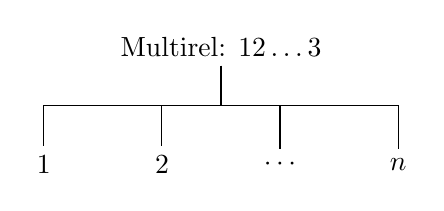
\begin{tikzpicture}
  \node {Multirel: $\rels1 \rels2 \ldots \rels3$}
    [edge from parent fork down]
    child {node {$\ex 1$}}
    child {node {$\ex 2$}}
    child {node {$\cdots$}}
    child {node {$\ex n$}}
    ;
\end{tikzpicture}


\subsection{Operator}

\textcolor{red}{The following might be rubbish\ldots}

The general operator rules are as follows:

\AXC{$A + B$}\RL{$infixop_1$}\UIC{+ A B}\DisplayProof\qquad 
\AXC{$\Phi + A$}\RL{$infixop_2$ with $\Phi\equiv + A_1\ldots A_n$}\UIC{$+ A_1 \ldots A_n A$}\DisplayProof 


\section{Schema}
\label{sec:schema}

A simple schema, ignoring attributes for the time being.

\begin{lstlisting}
<?xml version="1.0" encoding="utf-16"?>
<xsd:schema attributeFormDefault="unqualified" elementFormDefault="qualified" version="1.0" xmlns:xsd="http://www.w3.org/2001/XMLSchema">
  <xsd:element name="relseq" type="relseqType" />
  <xsd:complexType name="relseqType">
    <xsd:sequence>
      <xsd:element name="content" type="contentType" />
      <xsd:element name="children" type="childrenType" />
    </xsd:sequence>
  </xsd:complexType>
  <xsd:complexType name="childrenType">
    <xsd:sequence>
      <xsd:element maxOccurs="unbounded" name="infixop" type="infixopType" />
    </xsd:sequence>
  </xsd:complexType>
  <xsd:complexType name="infixopType">
    <xsd:sequence>
      <xsd:element name="content" type="contentType" />
      <xsd:element name="children" type="childrenType" />
    </xsd:sequence>
  </xsd:complexType>
  <xsd:complexType name="childrenType">
    <xsd:sequence>
      <xsd:element name="infixop" type="infixopType" />
      <xsd:element maxOccurs="unbounded" name="identifier" type="xsd:string" />
    </xsd:sequence>
  </xsd:complexType>
  <xsd:complexType name="infixopType">
    <xsd:sequence>
      <xsd:element name="content" type="contentType" />
      <xsd:element name="children" type="childrenType" />
    </xsd:sequence>
  </xsd:complexType>
  <xsd:complexType name="childrenType">
    <xsd:sequence>
      <xsd:element maxOccurs="unbounded" name="identifier" type="xsd:string" />
    </xsd:sequence>
  </xsd:complexType>
  <xsd:complexType name="contentType">
    <xsd:sequence>
      <xsd:element maxOccurs="unbounded" name="operator" type="xsd:string" />
    </xsd:sequence>
  </xsd:complexType>
</xsd:schema>
\end{lstlisting}



\section{Examples}
\label{sec:examples}


\subsection{Operators}
\label{sec:operators}

\subsubsection{Trivial}
\label{sec:trivial-ops}


\begin{lstlisting}
  <mi>a</mi>
  <mo>+</mo>
  <mi>b</mi>
  <mo>+</mo>
  <mi>c</mi>
\end{lstlisting}
\begin{lstlisting}
<infixop>+
  <content>
    <operator>+</operator>
    <operator>+</operator>
  </content>
  <children>
    <identifier>a</identifier>
    <identifier>b</identifier>
    <identifier>c</identifier>
  </children>
</infixop>
\end{lstlisting}



Simple Schema:
\begin{lstlisting}
<?xml version="1.0" encoding="utf-16"?>
<xsd:schema attributeFormDefault="unqualified" elementFormDefault="qualified" version="1.0" xmlns:xsd="http://www.w3.org/2001/XMLSchema">
  <xsd:element name="infixop" type="infixopType" />
  <xsd:complexType name="infixopType">
    <xsd:sequence>
      <xsd:element name="content" type="contentType" />
      <xsd:element name="children" type="childrenType" />
    </xsd:sequence>
  </xsd:complexType>
  <xsd:complexType name="childrenType">
    <xsd:sequence>
      <xsd:element maxOccurs="unbounded" name="identifier" type="xsd:string" />
    </xsd:sequence>
  </xsd:complexType>
  <xsd:complexType name="contentType">
    <xsd:sequence>
      <xsd:element maxOccurs="unbounded" name="operator" type="xsd:string" />
    </xsd:sequence>
  </xsd:complexType>
</xsd:schema>
\end{lstlisting}

\subsubsection{Combined}
\label{sec:combined-ops}


\begin{lstlisting}
  <mi>a</mi>
  <mo>+</mo>
  <mi>b</mi>
  <mo>+</mo>
  <mi>c</mi>
  <mo>-</mo>
  <mi>d</mi>
  <mo>-</mo>
  <mi>e</mi>
\end{lstlisting}
\begin{lstlisting}
<infixop>-
<content><operator>-</operator><operator>-</operator></content>
<children>
  <infixop>+
  <content><operator>+</operator><operator>+</operator></content>
  <children>
    <identifier>a</identifier>
    <identifier>b</identifier>
    <identifier>c</identifier>
  </children>
  </infixop>
  <identifier>d</identifier>
  <identifier>e</identifier>
</children>
</infixop>
\end{lstlisting}

Simple Schema:
\begin{lstlisting}
<?xml version="1.0" encoding="utf-16"?>
<xsd:schema attributeFormDefault="unqualified" elementFormDefault="qualified" version="1.0" xmlns:xsd="http://www.w3.org/2001/XMLSchema">
  <xsd:element name="infixop" type="infixopType" />
  <xsd:complexType name="infixopType">
    <xsd:sequence>
      <xsd:element name="content" type="contentType" />
      <xsd:element name="children" type="childrenType" />
    </xsd:sequence>
  </xsd:complexType>
  <xsd:complexType name="childrenType">
    <xsd:sequence>
      <xsd:element name="infixop" type="infixopType" />
      <xsd:element maxOccurs="unbounded" name="identifier" type="xsd:string" />
    </xsd:sequence>
  </xsd:complexType>
  <xsd:complexType name="contentType">
    <xsd:sequence>
      <xsd:element maxOccurs="unbounded" name="operator" type="xsd:string" />
    </xsd:sequence>
  </xsd:complexType>
</xsd:schema>
\end{lstlisting}



\subsection{Relations}
\label{sec:relations}

\begin{lstlisting}
  <mi>a</mi>
  <mo>=</mo>
  <mi>b</mi>
  <mo>=</mo>
  <mi>c</mi>
\end{lstlisting}

\begin{lstlisting}
<relseq>=
<content>
  <relation>=</relation>
  <relation>=</relation>
</content>
<children>
  <identifier>a</identifier>
  <identifier>b</identifier>
  <identifier>c</identifier>
</children>
</relseq>
\end{lstlisting}

\subsection{Mixed Operators and Relation}
\label{sec:operators-relations}

\begin{lstlisting}
  <mi>a</mi>
  <mo>+</mo>
  <mi>b</mi>
  <mo>+</mo>
  <mi>c</mi>
  <mo>-</mo>
  <mi>d</mi>
  <mo>-</mo>
  <mi>e</mi>
  <mo>=</mo>
  <mi>a</mi>
  <mo>-</mo>
  <mi>d</mi>
  <mo>+</mo>
  <mi>b</mi>
  <mo>+</mo>
  <mi>c</mi>
  <mo>-</mo>
  <mi>e</mi>
  <mo>=</mo>
  <mi>a</mi>
  <mo>+</mo>
  <mi>b</mi>
  <mo>-</mo>
  <mi>d</mi>
  <mo>-</mo>
  <mi>e</mi>
  <mo>+</mo>
  <mi>c</mi>
\end{lstlisting}

\pagebreak
\scriptsize
\begin{lstlisting}
  <relseq>
    =
    <content>
      <relation>=</relation>
      <relation>=</relation>
    </content>
    <children>
      <infixop>
        -
        <content>
          <operator>-</operator>
          <operator>-</operator>
        </content>
        <children>
          <infixop>
            +
            <content>
              <operator>+</operator>
              <operator>+</operator>
            </content>
            <children>
              <identifier>a</identifier>
              <identifier>b</identifier>
              <identifier>c</identifier>
            </children>
          </infixop>
          <identifier>d</identifier>
          <identifier>e</identifier>
        </children>
      </infixop>
      <infixop>
        -
        <content>
          <operator>-</operator>
        </content>
        <children>
          <infixop>
            +
            <content>
              <operator>+</operator>
              <operator>+</operator>
            </content>
            <children>
              <infixop>
                -
                <content>
                  <operator>-</operator>
                </content>
                <children>
                  <identifier>a</identifier>
                  <identifier>d</identifier>
                </children>
              </infixop>
              <identifier>b</identifier>
              <identifier>c</identifier>
            </children>
          </infixop>
          <identifier>e</identifier>
        </children>
      </infixop>
      <infixop>
        +
        <content>
          <operator>+</operator>
        </content>
        <children>
          <infixop>
            -
            <content>
              <operator>-</operator>
              <operator>-</operator>
            </content>
            <children>
              <infixop>
                +
                <content>
                  <operator>+</operator>
                </content>
                <children>
                  <identifier>a</identifier>
                  <identifier>b</identifier>
                </children>
              </infixop>
              <identifier>d</identifier>
              <identifier>e</identifier>
            </children>
          </infixop>
          <identifier>c</identifier>
        </children>
      </infixop>
    </children>
  </relseq>
\end{lstlisting}

\section{Examples}

\begin{lstlisting}
<math>
  <mi>5</mi>
  <mo>=</mo>
  <mi>3</mi>
  <mo>+</mo>
  <mi>2</mi>
</math>

<stree>
  <relseq role="equality" id="6">
    =
    <content>
      <relation role="equality" id="1">=</relation>
    </content>
    <children>
      <number role="integer" font="italic" id="0">5</number>
      <infixop role="addition" id="5">
        +
        <content>
          <operator role="addition" id="3">+</operator>
        </content>
        <children>
          <number role="integer" font="italic" id="2">3</number>
          <number role="integer" font="italic" id="4">2</number>
        </children>
      </infixop>
    </children>
  </relseq>
</stree>

<math>
  <mrow semantic-type="relseq" semantic-role="equality" id="6" semantic-content="1" semantic-children="0,5">
    <mi semantic-type="number" semantic-role="integer" id="0" semantic-parent="0">5</mi>
    <mo semantic-type="relation" semantic-role="equality" id="1" semantic-operator="=" semantic-parent="1">=</mo>
    <mrow semantic-type="infixop" semantic-role="addition" id="5" semantic-content="3" semantic-children="2,4" semantic-parent="5">
      <mi semantic-type="number" semantic-role="integer" id="2" semantic-parent="2">3</mi>
      <mo semantic-type="operator" semantic-role="addition" id="3" semantic-operator="+" semantic-parent="3">+</mo>
      <mi semantic-type="number" semantic-role="integer" id="4" semantic-parent="4">2</mi>
    </mrow>
  </mrow>
</math>
\end{lstlisting}

\end{document}

